\documentclass[a4paper]{article}
%%%%%%%% CREATE DOCUMENT STRUCTURE %%%%%%%%
%% 语言与编码格式
\usepackage{ctex}
\usepackage{babel}
\usepackage[utf8x]{inputenc}
\usepackage[T1]{fontenc}
\usepackage{subfig}

%% 设置页面页边距
\usepackage[a4paper,top=3cm,bottom=2cm,left=2cm,right=2cm,marginparwidth=1.75cm]{geometry}

%% 常用的包
\usepackage{amsmath}
\usepackage{graphicx}
%\usepackage{float}  %设置图片浮动位置的宏包
%\usepackage{subfigure}  %插入多图时用子图显示的宏包
\usepackage[colorinlistoftodos]{todonotes}
\usepackage[colorlinks=true, allcolors=blue]{hyperref}
\usepackage{caption}
%\usepackage{subcaption}
%\usepackage{subfigure}
\usepackage{sectsty}
\usepackage{apacite}
\usepackage{float}
\usepackage{titling} 
\usepackage{blindtext}
\usepackage[square,sort,comma,numbers]{natbib}
\usepackage[colorinlistoftodos]{todonotes}
\usepackage{xcolor}
\usepackage{setspace}
\usepackage{enumerate}
\usepackage{fontspec}
\usepackage{bm}
\definecolor{darkgreen}{rgb}{0.0, 0.4, 0.0}

%%%%%%%% DOCUMENT %%%%%%%%
\begin{document}
\bibliographystyle{unsrt}
%%%% 标题页
\begin{titlepage}

\newcommand{\HRule}{\rule{\linewidth}{0.5mm}} 							% horizontal line and its thickness
\center 
 
% 学校信息
\textsc{\LARGE 大连理工大学}\\[1cm]

% 文件信息
\textsc{\Large 专业方向课程设计大作业}\\[0.2cm]

\HRule \\[0.8cm]
{ \huge \bfseries 跨域手势识别的研究}\\[0.7cm]								
\HRule \\[2cm]

\large

\emph{姓名:}\ 金\quad \quad 田  \\
\emph{班级:}\ 网安1901\\
\emph{学号:} 201992268\\[1.5cm]													% 作者信息
{\large \today}\\[5cm]


\includegraphics[width=0.6\textwidth]{images/dlut.png}\\[1cm] 	% 学校logo
\vfill 
\end{titlepage}


\setmainfont{Times New Roman}

\tableofcontents

\clearpage

\section{课题背景}
\subsection{传统模式和发展现状}
  在智能技术领域中,人们持续致力于探索与智能设备更简便更精准的交互方式。在如今人机交互的方式越来越多样化的趋势下,人体姿态和手势的识别成为一个重要发展方向。\par
  手势是人类非语言类型中通俗易懂的一种表达形式,也可以作为人机交互的一种方式。在早期的智能家居模式下,已经可以实现用简单手势来操作一些电器和办公设备。在现有解决方案下已经有很多手势识别方式,其应用场景也各有不同,下面列举了三种典型的手势识别方法。 \par
  第一种是借助专门的传感器设备来获取信息,并建立相应的手势模型来进行手势识别。这种方式需要用户佩戴专门的设备进行数据提取,通过分析图像、声音等信息,借助已有的分类模型来分辨其行为。然而佩戴设备无疑增大了设备的使用成本,极大地降低了方便性。\par
  第二种是基于视频的手势识别,即利用摄像机来采集手势动作的视频,然后再根据视频数据提取手势特征完成手势识别。这种方法也有其局限性,容易受到光照、角度、分辨率等因素的影响,降低准确度,另外,视频数据的不确定性有时会涉及隐私问题,引起不必要的纠纷。\par
  第三种是基于无线射频的手势识别,也是最接近于目前主流技术的手势识别方法,其过程主要是在特定设备上获取手势动作的信号,对数据进行预处理后对手势进行分类。目前该方向的负面作用较小,有利于持续的研究发展。\par
  随着无线通信技术的快速发展,WIFI信号也为手势识别的数据来源带来了一种可能。WIFI信号在空间传播的过程中会由于用户的手势动作而产生多径传播的叠加效应,可以借助WIFI信号的波动情况识别出用户的手势动作。在利用WIFI信号进行手势识别时,对用户本身没有额外的要求,既不需要佩戴各种智能设备,也不会受到温度、光照条件的影响。目前基于WIFI的智能设备已经在实际生活和办公场景中广泛使用,这为WIFI环境下的手势识别信息研究提供了基础,通过WIFI信号来进行手势识别已经成为无线感知的热门技术之一\citep{gesture}。
  \subsection{弊端及创新点}
  在早期的基于无线感知技术的手势识别是从WIFI信号中提取物理特征并进行处理映射到手势动作,这些从WIFI信号直接提取到的特征包括了大量的环境因素,即会干扰正常手势引起信号波动的数据信息,这些信息会混杂在WIFI信号提取的信息中难以提取出来,一方面给纯粹的手势识别处理带来困难,另一方面映射的手势动作只局限于当时所处的实验环境,包括所处空间的结构、用户做手势的位置和方向,都会对结果产生较大影响。所以一旦设备所处的环境改变,就会面临原本功能失效的结果。在业界中,把与手势特征无关的因素(位置、信号强弱、空间分辨)成为“域”。各个科研团队持续研究的重点和难点是如何尽可能地消除环境给手势识别带来的影响,也就是让手势识别模型尽可能在不同的域之间保持稳定的识别准确率。\par
  因此在手势识别的研究中,最大的创新点在于从原始的与域相关的信号中提取仅反映手势本身与域无关的特征。近年来也有不少团队研究了一些成果,2017年,Chen等人通过online-independent SVM (OISVM)算法,SVM的参数,识别出环境变化后的动作。2018年,Yang等人提出的FALAR系统实现了自适应位置无关的活动识别,该系统利用基于核密度估计的运动提取方法和一种从粗到细的搜索策略来进行快速识别,无需考虑周围的环境。2019年,也是手势识别领域中具有飞跃性的一个阶段,清华大学团队设计了基于WIFI的跨域手势识别系统Widar,在较低信号水平上导出估计手势的速度曲线并形成BVP文件,这些数据表示手势的独特动力学特性,与环境并无关联,只需训练一次即可准确识别不同环境中的手势动作。该手势识别系统也作为本次课程报告的研究重点。
  \section{环境部署}
  在这一部分,将列举本次实际操作用到的一些工具的使用情况、环境配置以及数据集的详细信息。
  \subsection{工具}
  \subsubsection{Anaconda}
  随着深度学习算法的发展,衍生出了许多具有稳定架构的深度学习框架。现有的深度学习框架能够大幅度降低初学者的学习成本,通过实践发现,这些深度学习框架往往对编程语言和依赖包的版本有所要求。在大多数情况下,在某一环境下的深度学习框架不能在其他训练要求下生效,因此在执行不同的学习任务时,需要频繁地进行版本切换。\par
  Anaconda工具的出现就很好地解决了这个问题,Anaconda 是一个提供 Python 开发所需的工具包,包括 Python / IPython / CPython / Conda 等 180 个依赖项,同时支持 Linux,Mac,Windows 三大平台。有了Anaconda,依赖包的安装会简便许多。然而使用此工具的核心在于:Anaconda能够创建虚拟环境,可以针对不同的学习任务配置相应的包的版本。比如在一个学习任务中要求编程语言python 3.7,而另一个学习任务中要求python的版本为3.5,并且版本之间相互不兼容。在传统做法上,我们通常会修改现有的环境版本,这样做不仅过程十分繁琐,还可能因考虑不周出现依赖包残余,影响下一步的学习任务。有了Anaconda,只需要创建两个虚拟环境,编程语言和依赖包设置两个任务要求的版本,并且两个虚拟环境不存在冲突的情况,更有利于多学习任务的执行。下图展示了Anaconda安装之后的界面,表面上与cmd控制面板一致,同时会多一些conda的控制命令。\par
              \begin{figure}[H]
                \centering
                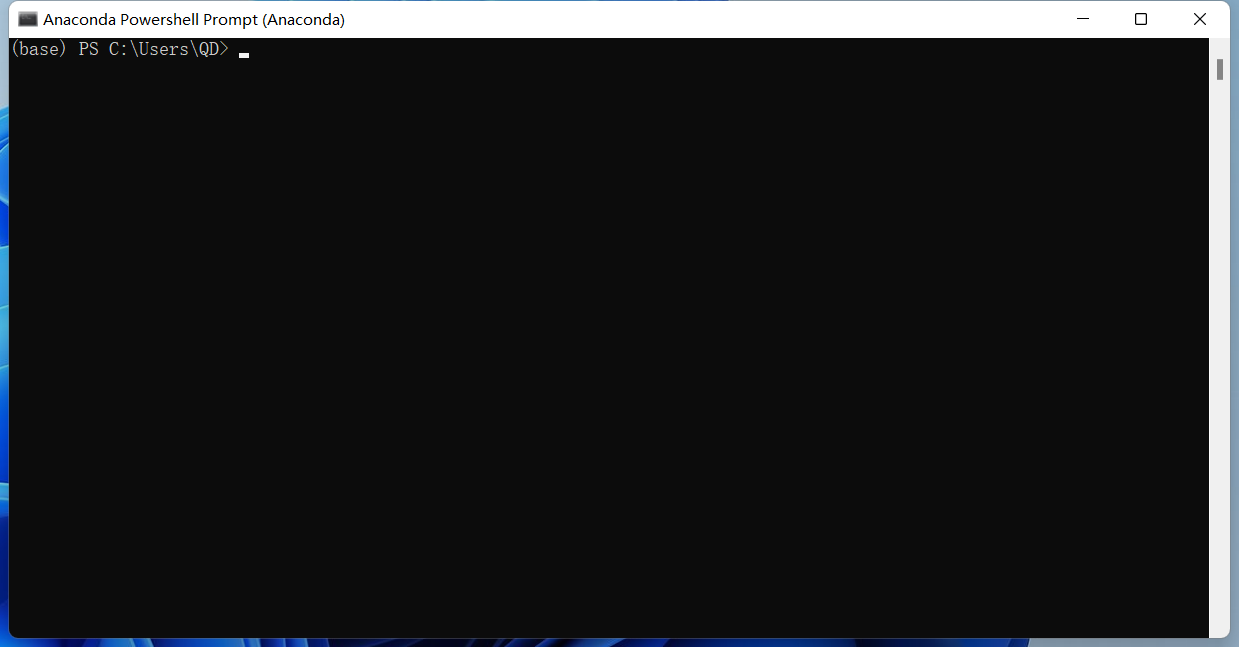
\includegraphics[width=16cm]{images/Anaconda.png}
                \captionsetup{font={small,bf,stretch=1.25}}
                \caption{Anaconda界面}
                \label{fig1}
            \end{figure}
  \subsubsection{Emacs}
  Emacs是小学期课程任务的重点,也是本次实践操作最常用的书写、编码工具。Emacs本质上和vim的定位一样,是一个古老而功能强大的专业编辑器。在Emacs的编辑器系列分支中,其中最主流的一支是 GNU Emacs,本次使用的 Emacs 也是指 GNU Emacs。\par
  \begin{figure}[H]
                \centering%居中
                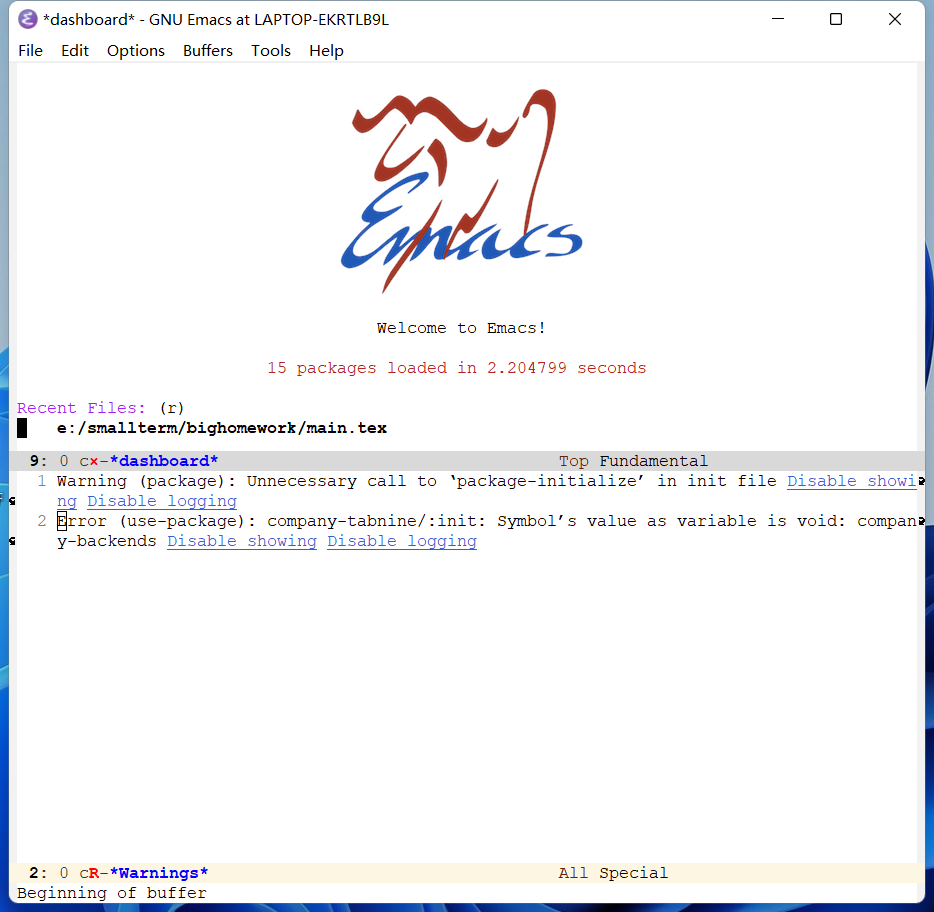
\includegraphics[width=12cm]{images/Emacs.png}
                \captionsetup{font={small,bf,stretch=1.25}}%图注格式设置
                \caption{GNU Emacs初始界面}
                \label{fig1}%标签,该图引用格式  \ref{fig1}
            \end{figure}
  Emacs能够在当前大多数操作系统上运行,包括类Unix系统(GNU/Linux、各种BSD、Solaris、AIX、IRIX、Mac OS X等等)、MS-DOS、Microsoft Windows以及OpenVMS等,还有移动Android平台以及iOS。Emacs依靠键盘的快捷键可以实现对文本、文件、代码的任意操作,图中整合了Emacs的常用操作,其中绝大多数的指令已经在实际操作中使用到。\par
            \begin{figure}[H]
	\centering
	\begin{minipage}{0.49\linewidth}
		\centering
		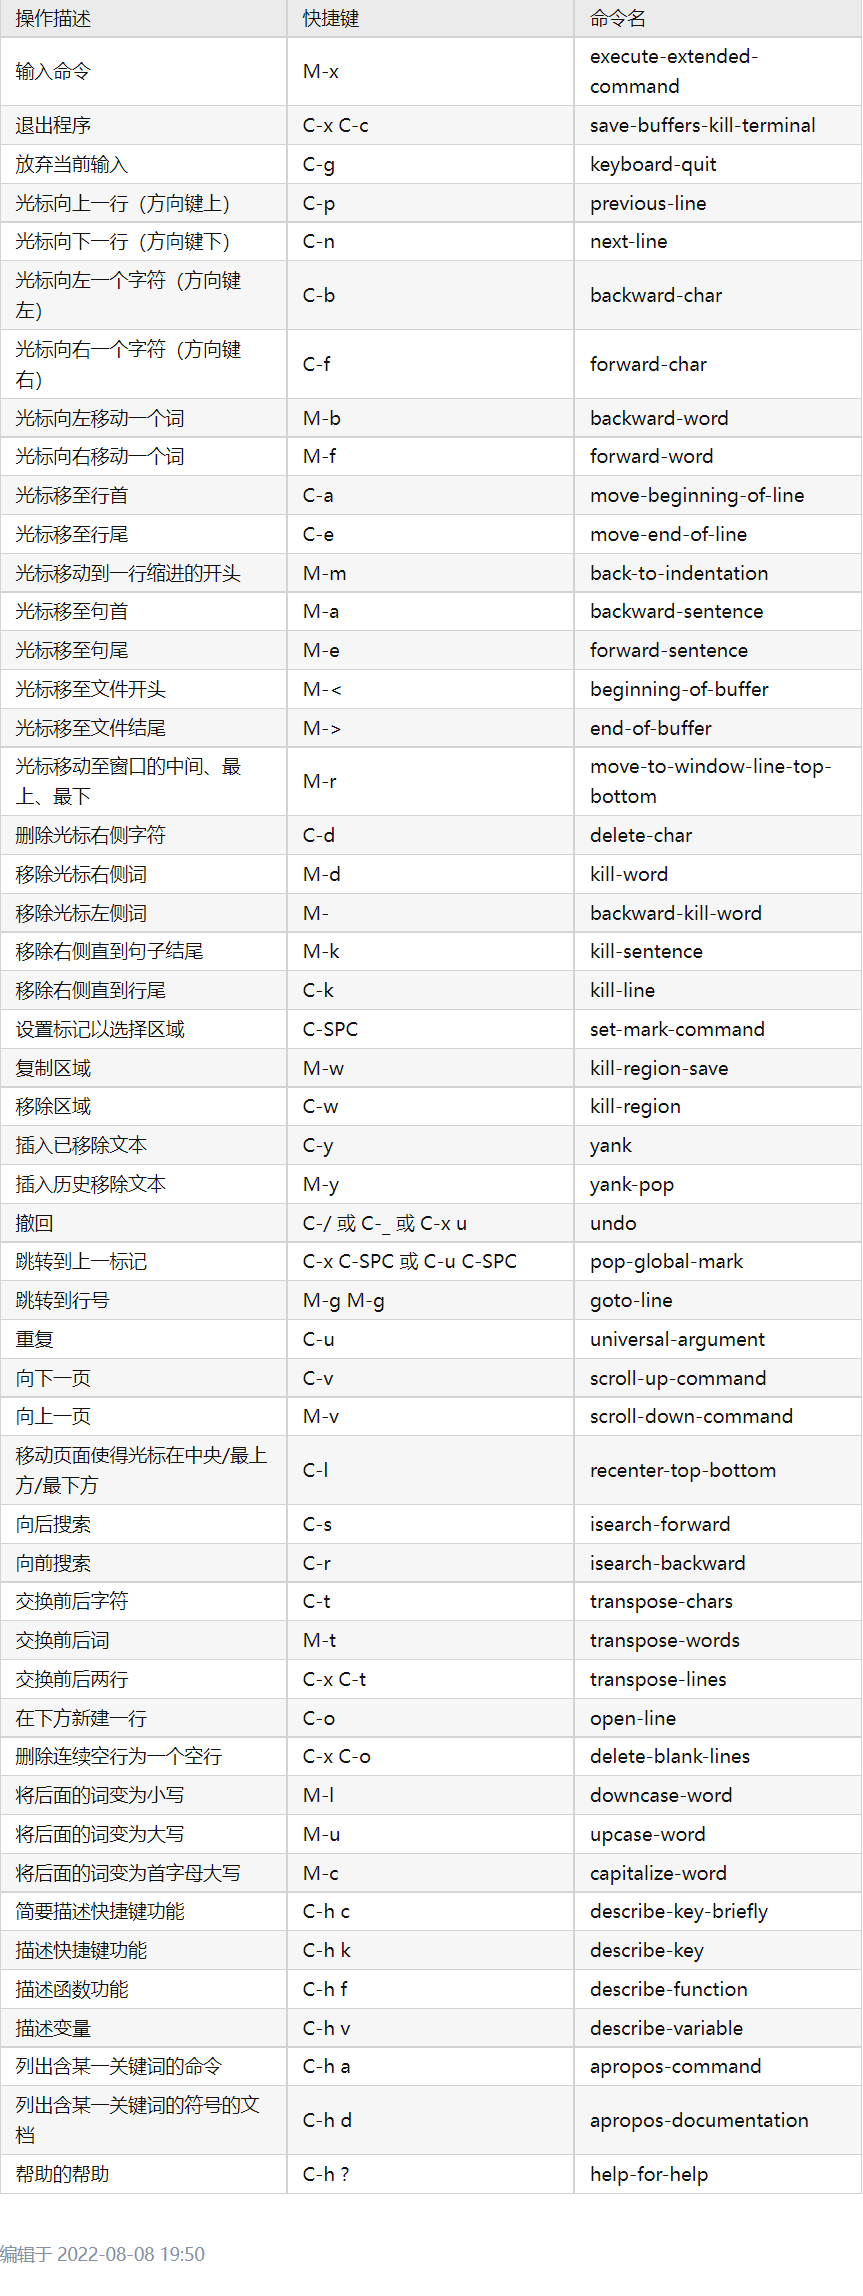
\includegraphics[width=6cm,height=15cm]{images/Emacs快捷键.png}
		\caption{Emacs快捷键}
		\label{fig1}%文中引用该图片代号
	\end{minipage}
	%\qquad
	\begin{minipage}{0.49\linewidth}
		\centering
		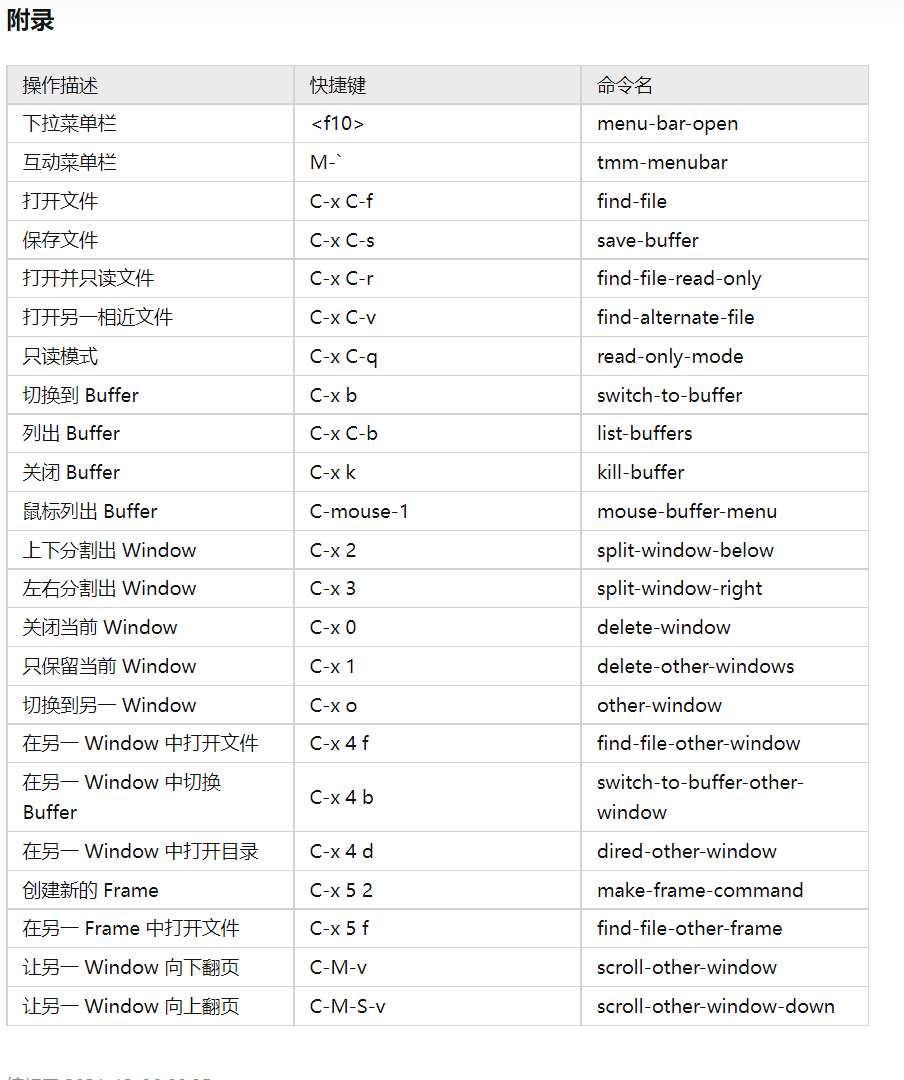
\includegraphics[width=6cm,height=15cm]{images/Emacs快捷键续.png}
		\caption{Emacs快捷键续}
		\label{fig1}%文中引用该图片代号
	\end{minipage}
      \end{figure}
  下图展示了在学习中Emacs的一些使用场景。 \par
                \begin{figure}[H]
                \centering
                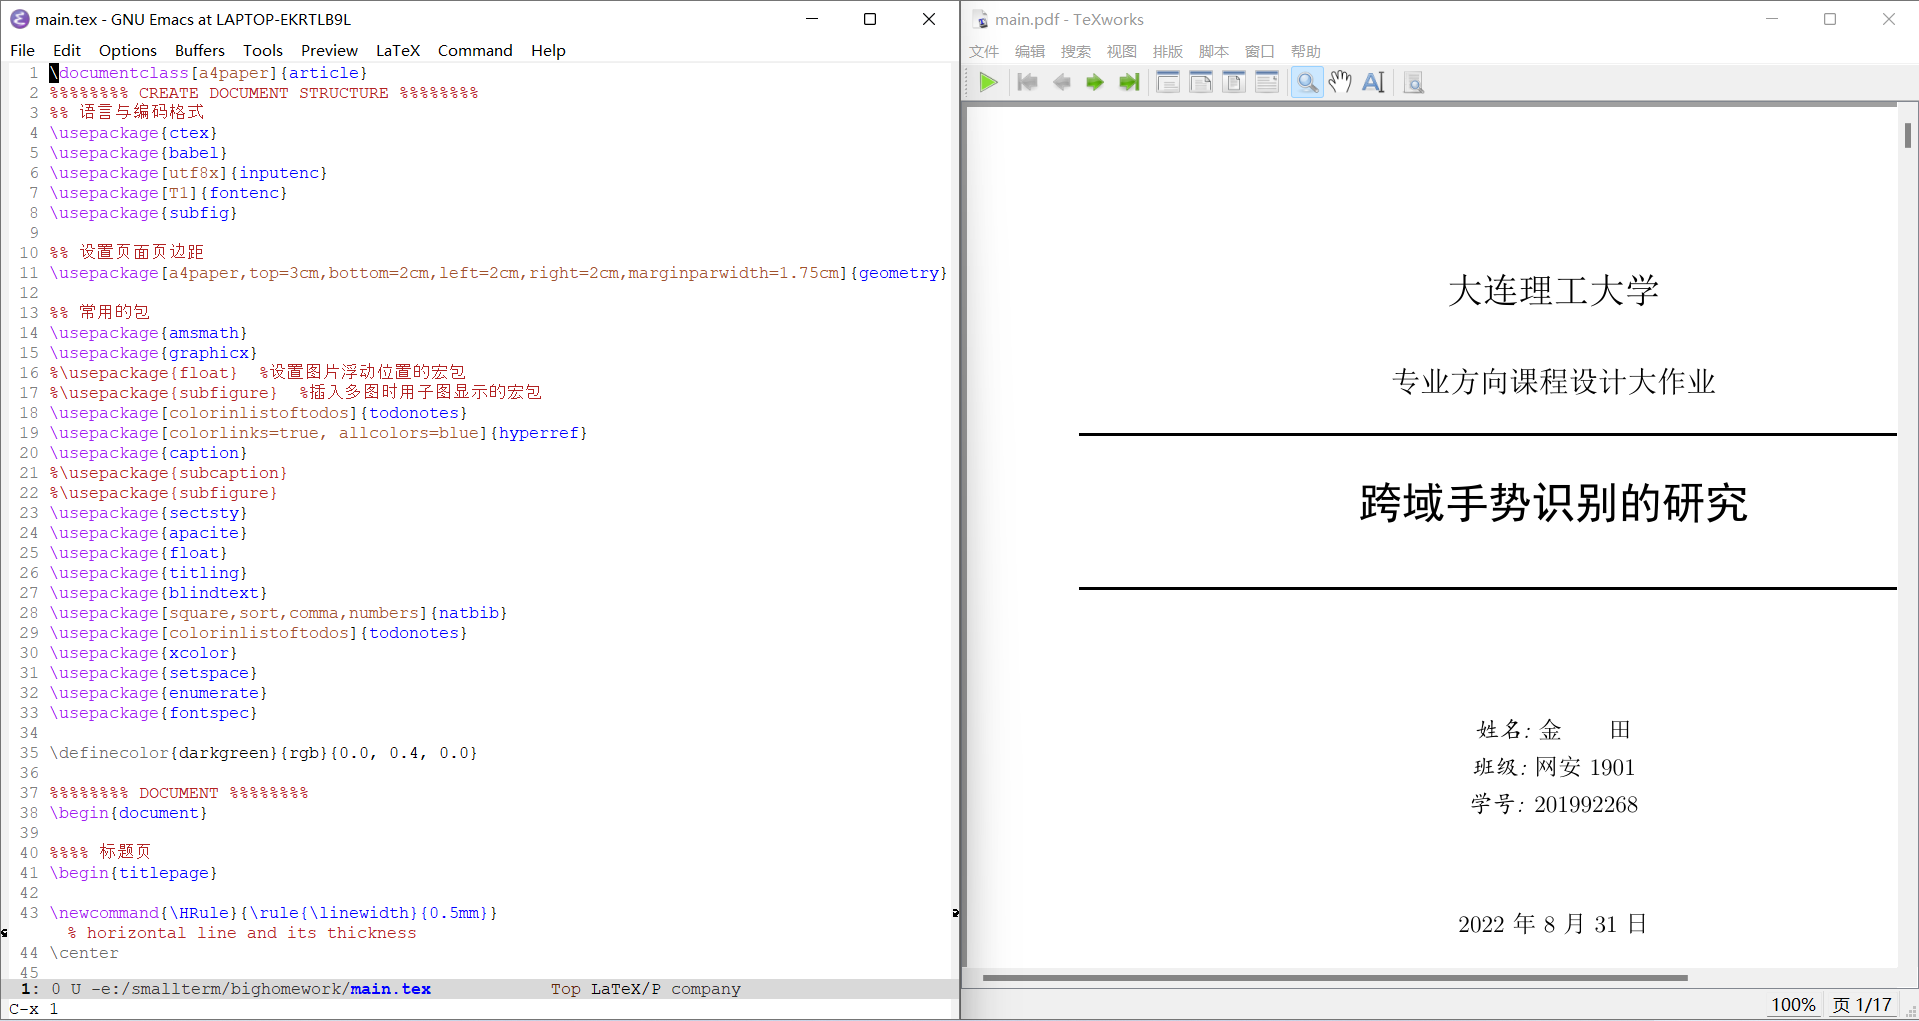
\includegraphics[width=16cm]{images/working.png}
                \captionsetup{font={small,bf,stretch=1.25}}
                \caption{Emacs Latex的桌面布置}
                \label{fig1}
              \end{figure}
                \begin{figure}[H]
                \centering
                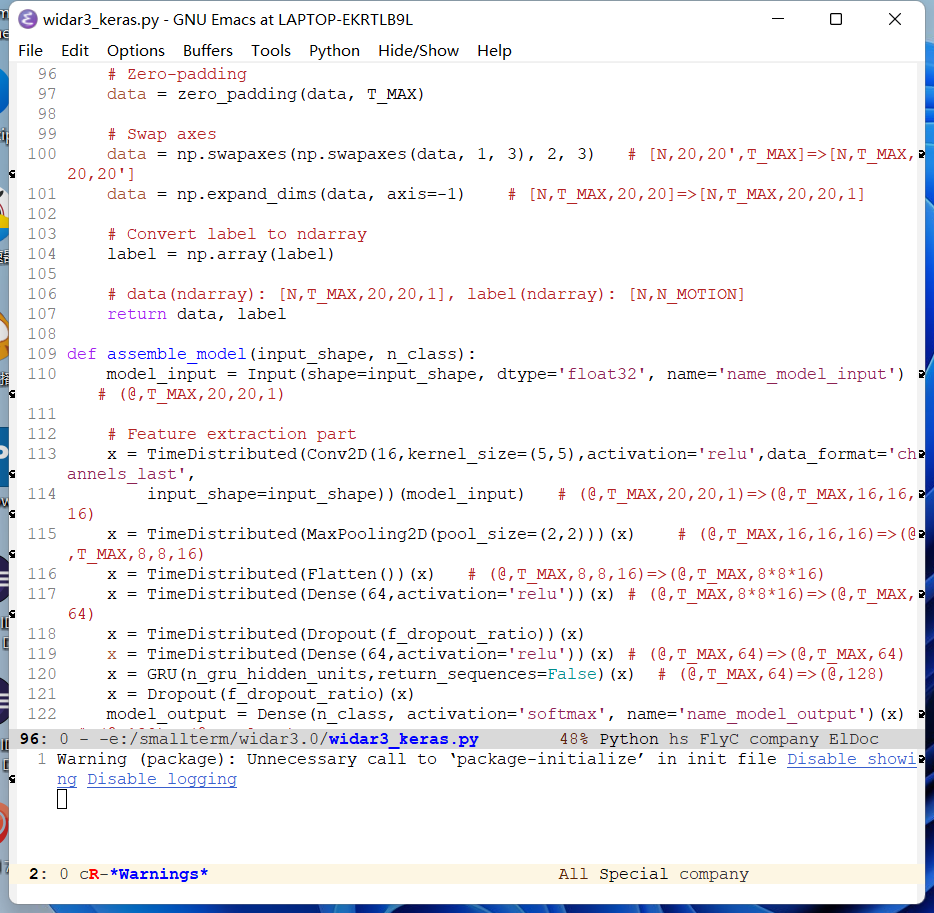
\includegraphics[width=16cm]{images/Emacs python.png}
                \captionsetup{font={small,bf,stretch=1.25}}
                \caption{Emacs python代码编写}
                \label{fig1}
              \end{figure}
  Emacs本身能实现的功能已经十分丰富,加上各个专业人员和编辑爱好者开发的插件,使Emacs强大的扩展性得以体现,这一古老的专业编辑器直到现在还焕发活力、经久不衰。在官方文档和其他参考资料中提到的功能优化、功能增强、界面美化、编程开发类的插件已达上千种,所以可以根据自己的喜好及功能需要选取合适的插件增加使用体验。\par
  在本课程中,本人安装了一些必要的插件如下:\par
  \begin{enumerate}
                \item[·] use-package,一个管理其它插件的插件,这样在安装新插件的时候,可以借助use-package功能下的Lisp语言实现自动安装。
                \item[·] column-number-mode,在编辑器上显示列号,这是后续编写代码的必备插件,在深度学习模型代码报错时,通过列号能够快速找到代码的错误点,从而进行修改。
                \item[·] flycheck,一个在编程模式下的代码语法检查工具,有了use-package,可以直接用hook模式设置。
                \item[*] dashboard,一个新的欢迎界面,可以列出最近打开的项目、最近打开的文件等等。按下p或r就可以快速 跳转到相应小结里。还可以列出来标记过的书签、org-mode(Emacs 自带的一个强大的笔记系统)日程、自定义控件等。
                \item[*] company-tabnine,代码补全工具,是一个带有AI性质的插件,自动补全代码对编程语言初学者非常友好。
                \end{enumerate}
            \subsubsection{LaTeX}
  本次大作业报告使用LaTeX进行排版,LaTeX的前身是TeX,TeX 是由Donald Knuth创造的基于底层编程语言的电子排版系统。使用TeX可以对版面做精细的操作,生成精美的文档。TeX提供版面编辑的底层命令,但是使用时操作复杂,工作效率不高. TeX允许用这些底层命令定义出可以执行复杂操作的扩展命令. LaTeX是由Leslie Lamport开发的的TeX扩展命令集合。LaTeX通过整合常用的版面设置操作,降低排版的工作量和难度。LaTeX强大的排版功能,特别是对科技文档的支持,已经使它成为撰写科研论文的事实上的标准。并且在使用LaTeX进行排版时,工作者的专业性得以体现。 \par
  在安装配置上,我选取了TeX Live 2022作为启动和运行TeX文档生成系统的工具,并且TeX Live自身带有TeXworks编辑器,选取XeLaTeX进行编译后(由于报告采用中文编写,用XeLaTeX避免出现乱码问题),可以点击按钮直接生成pdf文件。但是为了加深对Emacs熟练度,还是采用Emacs编写LaTeX文档。在use-package的插件基础上,利用“M-x customize-group tex-command”命令打开LaTeX配置界面,修改 TeX Command List、Value Menu->name、LaTeX-command-style 字段就可以使用C-c C-c编译,C-c C-p C-p预览。另外,在Emacs上编写LaTeX文档也具有语法高亮的功能,使用体验上强于TeXworks。 \par
  下图展示了用LaTeX编写文档的界面。 \par
    \begin{figure}[H]
                \centering
                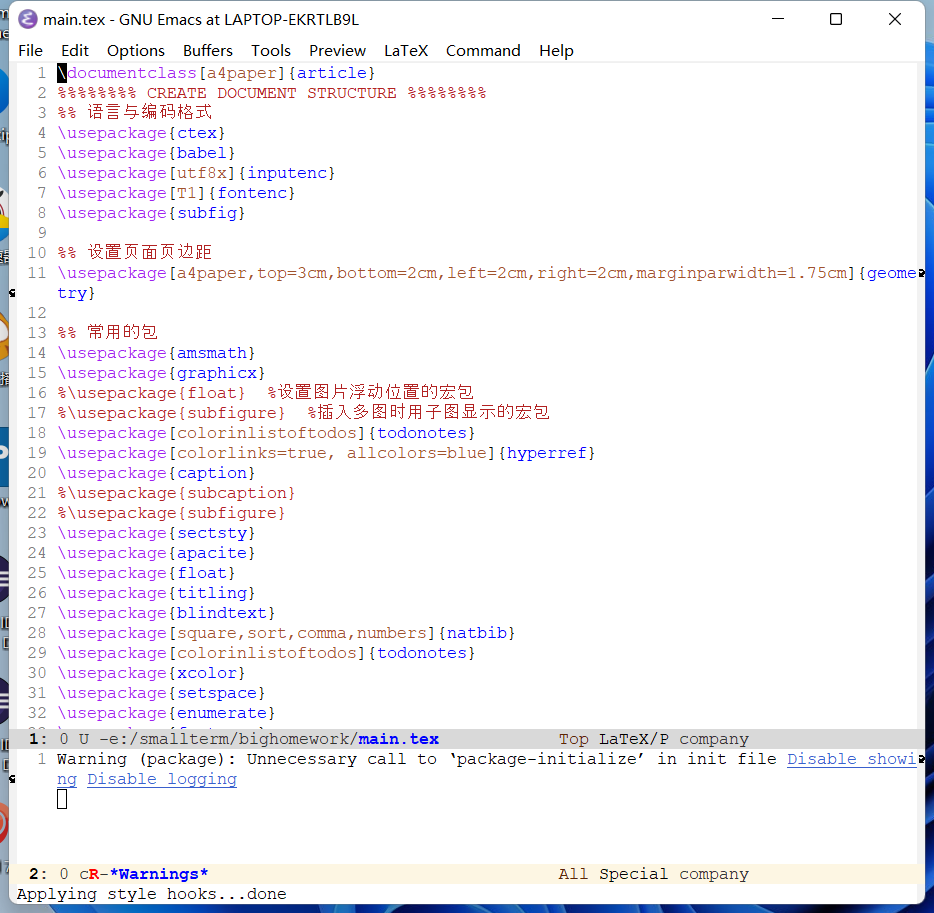
\includegraphics[width=16cm]{images/Emacs Latex.png}
                \captionsetup{font={small,bf,stretch=1.25}}
                \caption{Emacs LaTeX界面}
                \label{fig1}
              \end{figure}
  \subsection{环境}
  在本节中,会详细描述在手势识别领域创新点的产生过程和实验环境,它是理解跨域实现原理的基础。
  \subsubsection{pytorch}
  pytorch是一个基于torch的python开源机器学习库,用于自然语言处理等应用程序。作为一个很著名的支持GPU加速和自动求导的深度学习框架,在最近几年收到学术界的热捧,主要是因为其动态图机制符合思维逻辑,方便调试,适合于需要将想法迅速实现的研究者。pytorch运行速度虽然受动态图机制的影响没有tensorflow快,但是在GPU上的运行速度也是相当不错的。pytorch的安装也很简便,在Anaconda的基础上,创建符合CPU和显卡CUDA的版本的虚拟环境,利用官网生成的cmd命令安装相关依赖包即可。 \par
  在本次大作业中,对pytorch进行了一个简单的了解,并试验了一些torch相关的函数,运行了简单的训练代码。在手势识别的研究中,实际使用的是tensorflow框架。
  \subsubsection{tensorflow(keras)}
  tensorflow(keras)是大作业的重点训练使用的框架,tensorFlow 是一个采用数据流图(data flow graphs),用于数值计算的开源软件库。tensorFlow 最初由Google大脑小组(隶属于Google机器智能研究机构)的研究员和工程师们开发出来,用于机器学习和深度神经网络方面的研究,但这个系统的通用性使其也可广泛用于其他计算领域。它是谷歌基于DistBelief进行研发的第二代人工智能学习系统。2015年11月9日,Google发布人工智能系统tensorFlow并宣布开源。tensorflow的命名来源于本身的原理,tensor(张量)意味着N维数组,flow(流)意味着基于数据流图的计算。tensorflow运行过程就是张量从图的一端流动到另一端的计算过程。张量从图中流过的直观图像是其取名为“tensorflow”的原因。tensorFlow的关键点是:“Data Flow Graphs”,表示tensorFlow是一种基于图的计算框架,其中节点(Nodes)在图中表示数学操作,线(Edges)则表示在节点间相互联系的多维数据数组,即张量(tensor),这种基于流的架构让tensorFlow具有非常高的灵活性,该灵活性也让tensorFlow框架可以在多个平台上进行计算,例如:台式计算机、服务器、移动设备等。 \par
  keras是基于tensorFlow和theano(可以理解为tensorflow与keras的中间框架)的深度学习库,是由纯python编写而成的高层神经网络API,也仅支持python开发。它是为了支持快速实践而对tensorflow或者theano的再次封装,让使用者可以不用关注过多的底层细节,能够把想法快速转换为结果。keras默认的后端为tensorflow,在这里可以看出keras和tensorflow是一个包含的关系。如果用到theano可以自行更改。tensorflow和theano都可以使用GPU进行硬件加速,往往可以比CPU运算快很多倍。因此如果显卡支持cuda的话,会利用cuda加速模型训练。
  \subsection{数据集}
  大作业研究的主要内容是在2019年清华大学科研团队推出的Widar3.0数据集。在以往的模型训练上,普遍都缺乏对跨域的自适应工作,因此当出现新的数据域时,无论是数据收集还是模型重新训练,都需要额外的训练工作,带来较大的开销,从而限制了其实用性。Widar3.0的核心思想是在较低信号水平上推导和估计手势的速度分布,这代表了手势的独特动力学特征并且与域无关。Widar3.0利用卷积神经网络与循环神经网络分别挖掘输入特征BVP在空间维度与时间维度的特性,对6种常见的人机交互手势(推拉、横扫、拍手、滑动、画圆、画之字)进行判别。另外,还开发了一种只需要一次性训练但可以适应不同数据域的万能模型。在不同域间的识别准确率也能达到92.4\%。因此Widar3.0的亮点不在于训练模型,而在于对手势相关和手势无关数据的提取。\par
  该数据集包总共大小达325GB,包括了2018~2019年的若干次实验数据,其中BVP生成模块含有CSI原始数据、DFS配置文件及转化算法和BVP数据及转化算法;手势识别模块实现了用于手势识别的深度学习神经网络(DNN)。Widar3.0处理的是生成的BVP数据,对每个BVP以及整个系列进行归一化操作,以去除实例和人员的不相关变化。然后将归一化的BVP系列输入到时空DNN中,该DNN具有两个主要功能。首先DNN利用卷积层从每个BVP中 \textbf{提取高级空间特征}。然后采用循环层对BVP之间的相互特征进行 \textbf{时间建模}。最后,DNN的输出用于指示用户执行的手势类型。Widar3.0原则上实现了跨域手势识别的通用模型,只需要对该深度神经网络网络进行一次训练,就可以在域间保持较高的准确率。\par
  另外,有必要对数据集中的三个重要数据类型作出定义。 \par
    \begin{enumerate}
  \item[·] CSI(Channel State Information):信道状态信息,CSI是信号在传输过程中利用OFDM技术得到的能够表示物理层细粒度的信号特征。在无线通信领域,CSI指的是通信链路的信道属性。它描述了信号在每条传输路径上的衰弱因子,即信道增益矩阵H中每个元素的值,如信号散射(Scattering),环境衰弱(fading,multipath fading or shadowing fading),距离衰减(power decay of distance)等信息。CSI可以使通信系统适应当前的信道条件,在多天线系统中为高可靠性高速率的通信提供了保障。CSI信号的幅度信息可以量化多径效应后的信号功率衰减。因此,通过分析人体手势动作对信号造成的幅度和相位影响可以有效识别人类动作。
  \item[·] DFS(Doppler Frequency Shift):多普勒频移,指的是多普勒效应造成的发射源和接收源的频率之差。人的所有身体部位都有独特的速度分布,可以用作活动指标,在人反射信号的所有参数中,DFS体现了速度分布的大部分信息。当一个人做一个手势时,他的身体部位(例如,两只手、两只手臂和躯干)以不同的速度移动。因此,这些身体部位反射的信号会经历各种DFS,这些DFS在接收器处叠加并形成相应的DFS轮廓。通过计算同一Wi-FiNIC上两个天线的CSI的共轭乘法,并滤除带外噪声和准静态偏移,可以去除随机偏移,并且只保留具有非零DFS的显着多径分量。进一步应用短期傅立叶变换会产生时间和多普勒频域上的功率分布。具体来说,DFS配置文件D是一个维度为F×M的矩阵,其中F是频域中的采样点数,M是收发器链路数。基于来自多个链接的DFS配置文件,最终可以形成BVP数据。
  \item[·] BVP(Body-coordinate Velocity Profile):身体坐标速度分布文件,它描述了不同速度上的功率分布,其中身体部位参与了手势运动。我们的观察是,无论在哪个域中做出手势,每种类型的手势在身体坐标系中都有其独特的速度分布。因此,这些身体部位反射的信号会经历各种DFS,这些DFS在接收器处叠加并形成相应的DFS轮廓。虽然DFS配置文件包含手势信息,但它也高度特定于域。相比之下,人的身体坐标系中物体速度的功率分布仅与手势的特征有关。因此,为了消除域的影响,BVP是从DFS配置文件中派生出来的。
  \end{enumerate}
  \subsubsection{采集设备}
  Widar3.0由一个发射器和三个以上的接收器组成,远端接收器的角度大于180°。所有收发器都是现成的迷你桌面(物体尺寸170mm×170mm),配备Intel5300无线网卡。Linux-CSI-Tool安装在设备上以记录CSI测量结果。设备设置为在监控模式下工作,在5.825GHz的165频道上,可以将干扰无线电减少到最小,因为干扰确实会对收集的CSI测量值造成严重影响。发射器激活一根天线并以每秒1,000个数据包的速率广播Wi-Fi数据包。接收器激活所有三个放置在一条线上的天线。并在MATLAB和Keras中实现了Widar3.0\citep{core}。 \par
   \begin{figure}[H]
	\centering
	\begin{minipage}{0.3\linewidth}
		\centering
		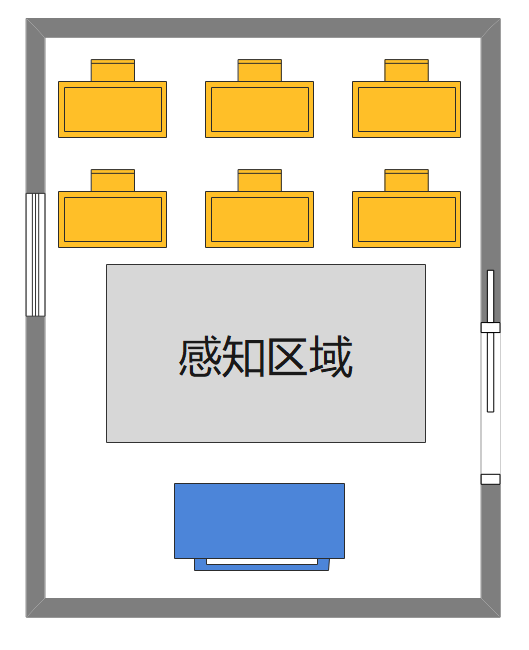
\includegraphics[width=4cm,height=4cm]{images/Room1.png}
		\caption{Room1}
		\label{fig1}
              \end{minipage}
              % \qquad
	\begin{minipage}{0.3\linewidth}
		\centering
		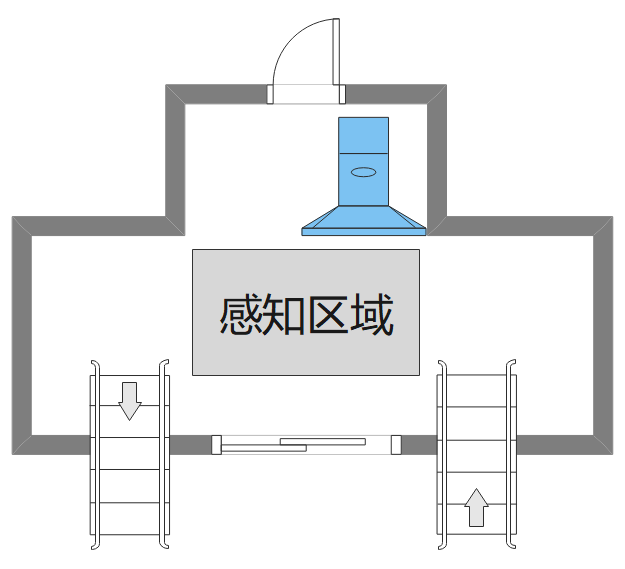
\includegraphics[width=4cm,height=4cm]{images/Room2.png}
		\caption{Room2}
		\label{fig1}
              \end{minipage}
              % \qquad
              \begin{minipage}{0.3\linewidth}
                \centering
                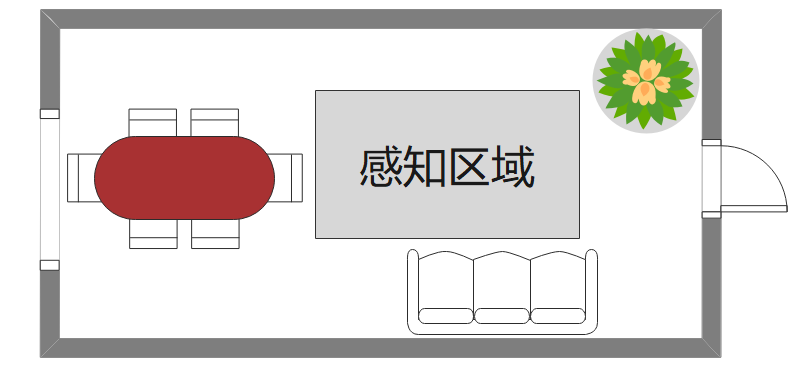
\includegraphics[width=4cm,height=4cm]{images/Room3.png}
                \caption{Room3}
                \label{fig1}
              \end{minipage} 
      \end{figure}
  在空间环境上,选取了三个门内环境进行广泛的手势识别实验,一个配有桌椅的空教室、一个宽敞的大厅和一个配有沙发和桌子等家具的办公室。配有桌椅的空教室处于一个常规的长方体空间,存在的智能设备功能广泛应用在教学中,其影响信号的因素在于多个桌椅带来的信号反射不规律性;宽敞的大厅呈“凸”字形,其结构虽然不如长方体空间带来的信号间接,但是其拥有的对称性也是有迹可循;配有沙发和桌子等家具的办公室相对于配有桌椅的空教室,其空间大小有所减小,家具数量少、体积大,也是智能设备最常存在的情况。这三个门内环境对于手势识别的评估很具有代表性。
  \subsubsection{采集过程}
  手势数据的采集流程和模型形成的步骤可以概括为下图所示。 \par
    \begin{figure}[H]
                \centering
                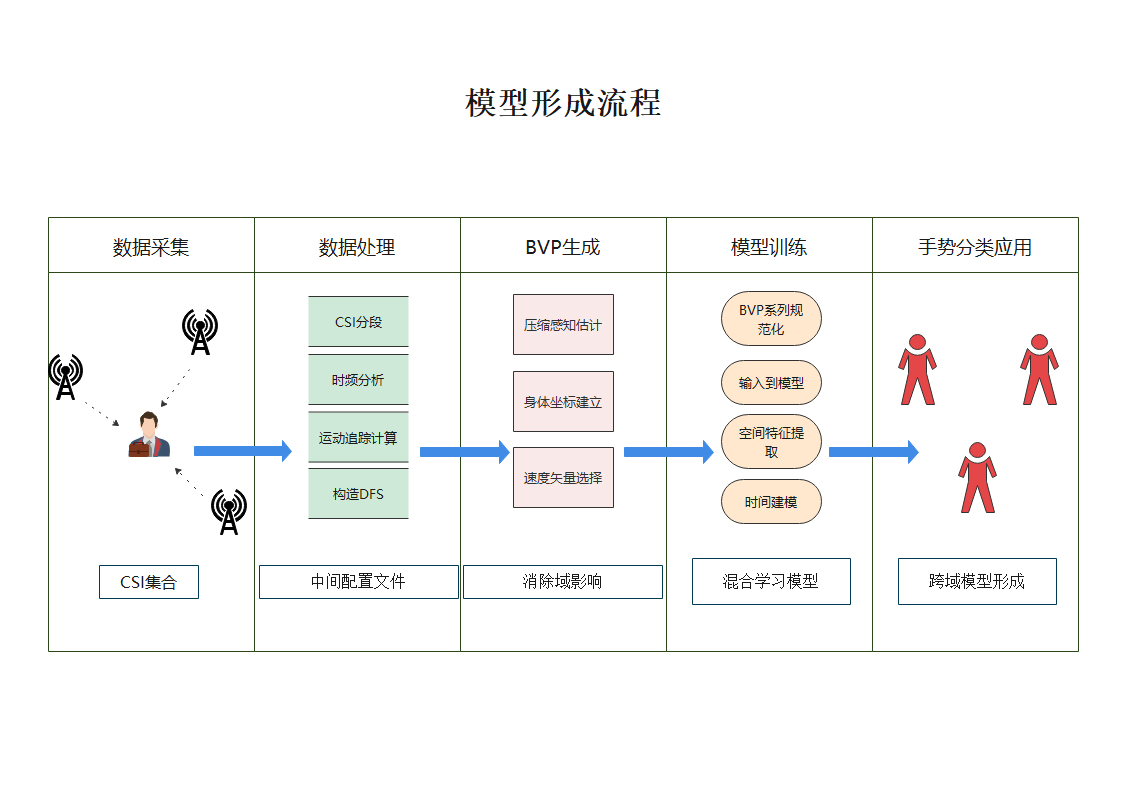
\includegraphics[width=16cm]{images/process.png}
                \captionsetup{font={small,bf,stretch=1.25}}
                \caption{模型形成过程}
                \label{fig1}
              \end{figure}
  在已存在WIFI设备的前提下,首先要进行手势数据的提取,在监控区域周围部署多条无线链路。在接收器处
采集用户在监控区域内失真的无线信号,并记录和预处理其CSI测量值。CSI描述了数据包到达时间t时室内环境中的多径效应,预处理的主要目的是消除幅度噪声和相位偏移. \par
  手势识别系统接收到净化后的CSI系列后,将CSI系列划分小段,用于分段生成BVP。在时频分析步骤中,要充分考虑路径数和相应的复衰减和传播延迟。通过用相应的DFS表示多径信号的相位,CSI可以转换为频谱形式,进一步产生时间和多普勒频域上的分布。之后,通过运动跟踪方法计算人的方向和位置信息,这里提出了身体坐标的概念,因为每种类型的手势在身体坐标系中都有其独特的速度分布,这也是导出速度分量的信号功率分布的前提,最后得到了人的方向、位置信息以及DFS配置文件,这些数据相当于BVP生成的中间文件\citep{gesture2}。 \par
  最关键的一步也是BVP数据文件的生成,当用户与设备进行交互时,会靠近它并进行交互手势来识别和响应。人的先前运动为估计位置和方向提供了机会,这些位置和方向是人在轨迹末端的位置和移动方向。由于基于Wi-Fi的被动跟踪已经被广泛研究,Widar3.0利用了现有复杂的被动跟踪系统,例如LiFS、IndoTrack和Widar2.0,来获取目标的位置和方向。然而,Widar3.0与这些被动跟踪方法的不同之处在于估计BVP而非主躯干速度,因此进一步扩展了基于Wi-Fi的传感范围。一个BVP被量化为维度为N×N的离散矩阵,其中N是沿身体坐标的每个轴分解的速度分量的可能值的数量。建立局部身体坐标,其原点是人的位置,正x轴与人的方向对齐。我们将在第4.4节讨论估计一个人的位置和方向的方法。目前,假设该人的全球位置和方向是可用的。然后可以将已知的无线收发器的全球位置转换为局部身体坐标。人体周围的速度分量将其信号功率贡献给对应的频率分量,由于在计算DFS配置文件之前过滤掉了具有零DFS的静态分量,因此只保留人的反射信号。当人靠近WIFI链路时,只有一次反射的信号具有明显的幅度,因此根据链路信息和速度分量可以对DFS与BVP之间的关系建立模型。由于单个手势的DFS文件变量达到数百个之多,而物理链路只能提供有限数量的约束,所以要利用反射多径信号的数量有限性以及DFS剖面带来的投影重叠,可以从有限的链路的DFS文件中正确恢复BVP。 \par
  在模型训练上,Widar3.0设计了一个DNN学习模型来挖掘BVP系列的时间和空间特征,该深度神经网络包含了用于空间特征提取的卷积神经网络(CNN)和用于时间建模的递归神经网络(DNN),这样的一个混合深度学习模型以前一步的BVP数据作为输入,实现准确的跨域手势识别。首先将BVP系列进行规范化处理,设置手势的标准时间长度,缩放BVP中所有速度分量的倍数,假设每个身体部位移动的总距离保持固定,将BVP系列进行时间缩放,之后将序列重新采样到原始BVP序列的采样率。这样经过规范化处理的输出数据仅与手势相关,将其输入到深度学习模型。 \par
  卷积神经网络提供了一种提取空间特征和压缩数据的实用技术,它可以用于处理高度稀疏但保留空间局部性的单个BVP,BVP类似于图像序列,单个BVP描述了在足够短的时间间隔内物理速度上的功率分布,连续的BVP系列说明了分布如何对应于某种动作的变化。输入的BVP系列作为维度为N*N*T的张量,其中T是BVP快照的数量,对于第t个采样的BVP,矩阵被馈送到CNN。在CNN中首先将16个2-D滤波器应用于V..t以获得速度域中的局部模式,从而形成输出v(1)..t,然后将最大池化应用于v(1)..t对特征进行采样,输出表示为v(2)..t。两个以ReLU作为激活函数的64单元密集层用于进一步提取更高级别的特征。在两个密集层之间添加了一个额外的dropout层以减少过度拟合。最终输出v..t表征第t个采样BVP,并且输出序列用作后续循环层的输入以进行时间建模。 \par
  除了每个BVP中的局部空间特征外,BVP系列还包含手势的时间动态。递归神经网络(RNN)的吸引力在于它们可以对复杂的序列时间动态进行建模。有不同类型的RNN单元,例如SimpleRNN、长短期记忆(LSTM)和门控循环单元(GRU)。与原始RNN相比,LSTM和GRU更适用于学习长期依赖关系,GRU在序列建模上实现了与LSTM相当的性能,但涉及的参数较少,并且更容易用更少的数据进行训练。Widar3.0采用单层GRU来建模时间关系,来自CNN的输入{v..t t=1...T}输出被馈送到GRU,并生成一个128维的向量。此外,为正则化添加了一个dropout层,并使用一个带有交叉熵损失的softmax分类器进行类别预测。
  经过了上述过程的模型训练,Widar3.0的整体准确率可达92.7\%,在Room1中收集的90\%和10\%的数据分别用于训练和测试。Widar3.0对所有手势均实现了超过85\%的高精度。我们还额外添加了“未知”类的手势进行实验。除上述6种手势外,志愿者需要进行任意手势。整体准确率下降到90.1\%,Widar3.0可以区分未知类,准确率达到87.1\%。来自未知类别的手势在一定程度上类似于预定义的手势,会使准确率没有下降得太多;收集到的未知手势数量仍然有限,未来如果引入额外得过滤机制或修改,结果可以进一步改善。

  \clearpage
  \section{实验操作}
  在本章节中,重点对模型训练部分的实践做出概述。
  \subsection{环境版本}
  深度学习环境以Anaconda作为依赖包资源和虚拟环境创建工具,Anaconda的版本并无硬性要求,所以安装了最新版本的Anaconda是可以投入使用的。 \par
  使用的深度学习框架为tensorflow和keras,其中keras相当于tensorflow的一个高阶应用程序接口,所以安装时尤其注重了版本之间的对应关系,后面的代码实现会体现tensorflow的简便性。在本机环境中tensorflow版本为2.0.0,对应了keras的版本为2.3.1,同时也对python的版本做出了范围要求,在创建虚拟环境时给出参数选取了python为3.6,实际安装版本为3.6.13,以上的搭建保证了代码正常运行的基础条件。其他附带的依赖包如下图所示。 \par
  \begin{figure}[H]
    \centering
    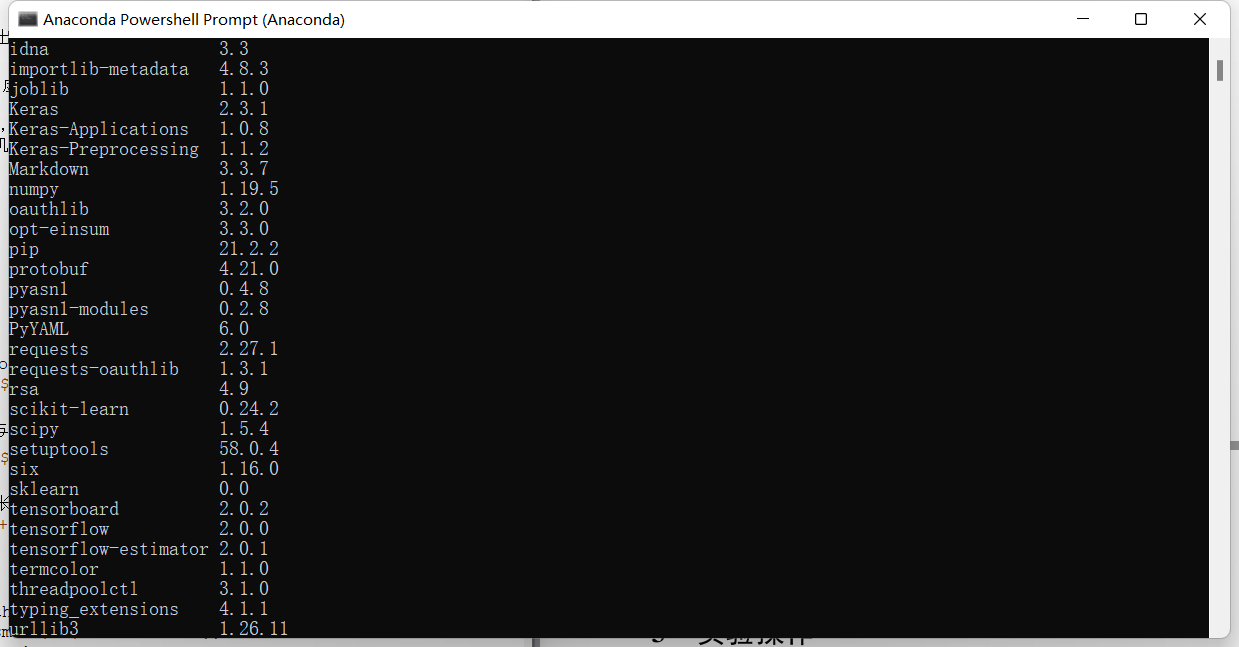
\includegraphics[width=16cm]{images/package.png}
    \captionsetup{font={small,bf,stretch=1.25}}
    \caption{该虚拟环境下需要安装的依赖包}
    \label{fig1}
  \end{figure}
  
  \subsection{硬件支持}
  在模型部署时,为了把握训练速度和精度,需要重点关注硬件设备。由于实验条件的限制,只能利用笔记本电脑的配置进行深度学习。
              \begin{enumerate}
                \item[.] CPU:Intel(R) Core(TM) i7-9750H CPU @,在2019年第二季度推出,拥有6核心12线程,主频2.60GHz,自带英特尔®超核芯显卡630,可以作为辅助GPU为训练加速处理。
                \item[.] GPU:NVIDIA GeForce RTX 2060, CUDA核心数量为2176,基础频率1.47GHz,加速频率1.65GHz,配有12GB GDDR6显存。
                \end{enumerate}
                以上配置可以保证本次手势识别深度学习的训练速度和准确度。
  \subsection{代码实现与调整}
  在提供的深度神经网络(DNN)模型代码中,运用了大量受版本限制的库和函数,在实践过程中可以判断中,本机使用版本与源代码实现版本不同且不兼容,进行后的调整后导入包如下图所示。 \par
              \begin{figure}[H]
                \centering
                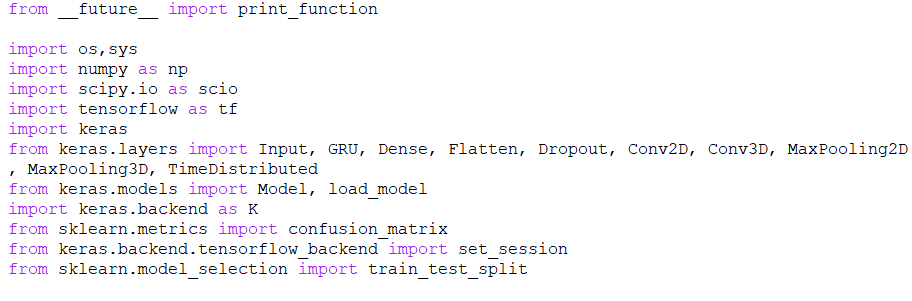
\includegraphics[width=16cm]{images/import.png}
                \captionsetup{font={small,bf,stretch=1.25}}
                \caption{import导入情况}
                \label{fig1}
              \end{figure}
  其中os,sys是系统模块,涉及到文件读取的操作需要用到;numpy主要是对数组进行转维和一些计算;scipy依赖于numpy,目的是进行便捷且快速的N维数组操作。 \par
  之后引入了tensorflow和keras模块,为了之后的张量计算和时间建模,同时还要引入Input、GRU(门控循环单元)、Dense等包。keras.models模块与模型建立有关,backend是keras默认支持的后端,在运行中会出现”Using tensorflow backend”字样。sklearn库用来进行自动参数调整和神经模型调参,sklearn.model\_selection中可实现的功能有构造数据的交叉验证迭代器以及拆分训练集与测试集。\par
  在训练前还需要设置一些参数如下图所示。\par
                \begin{figure}[H]
                \centering
                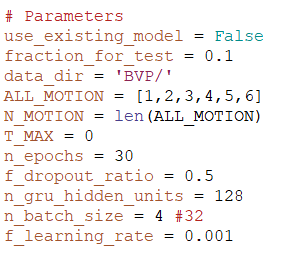
\includegraphics[width=8cm]{images/parameters.png}
                \captionsetup{font={small,bf,stretch=1.25}}
                \caption{预先设置的Parameters}
                \label{fig1}
              \end{figure}
  上述参数指定的一些内容为为:不利用已有的训练模型,设置了训练集与测试集的比例,规定了训练精度要求,指出了训练次数和每次训练样本数以及一些其他的单元数据。 \par           
  对于Widar3.0实验提供的参数,为了与本机配置环境兼容,做出了调整。首先,在之前的背景知识了解下明确该模型处理的是BVP数据,所以将data\_dir由先前的Data调整为BVP;由于在训练时发生了显存不足的错误,所以调整了n\_batch\_size从32下降到4,这样可以防止程序途中崩溃。\par
  训练步骤开始,首先提供了硬件选择的代码。 \par
                \begin{figure}[H]
                \centering
                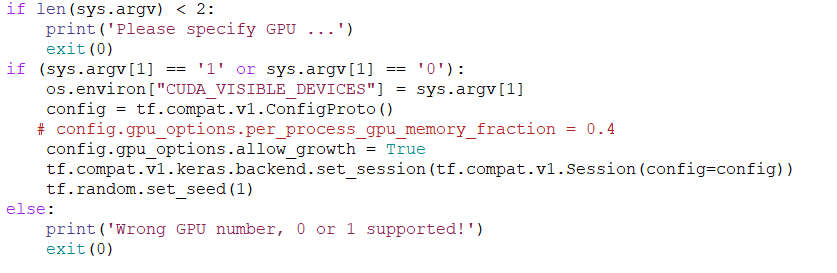
\includegraphics[width=12cm]{images/begin.png}
                \captionsetup{font={small,bf,stretch=1.25}}
                \caption{硬件选择}
                \label{fig1}
              \end{figure}
  从代码中的sys.argv可以看出,它给予用户硬件选择的机会,在运行python程序时需要给出选择的GPU,并作为os.environ["CUDA\_VISIBLE\_DEVICES"]的参数。config = tf.compat.v1.ConfigProto()配置了运算方式,这里进行了版本代码的调整。由于tensorflow默认会跑满整个内存,且之前的实践过程出现了多次的内存错误,调整GPU动态使用并不能解决问题,所以硬性地指定了GPU的使用比率,通过观察硬件使用情况得出结论:在使用40\%的GPU时效果较好。 \par
  基于keras的特征提取部分代码及损失函数如下图所示。 \par
                \begin{figure}[H]
                \centering
                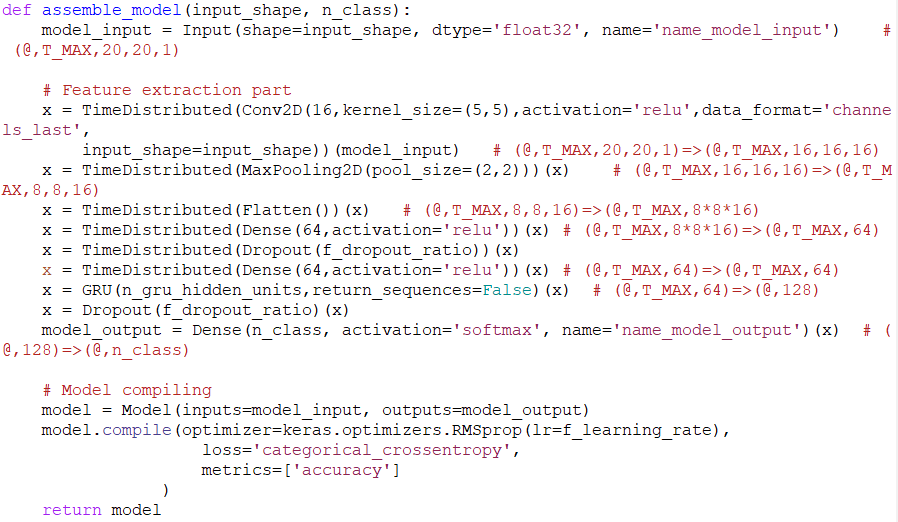
\includegraphics[width=12cm]{images/model.png}
                \captionsetup{font={small,bf,stretch=1.25}}
                \caption{特征提取参数和损失函数}
                \label{fig1}
              \end{figure}
  该特征提取部分也是keras框架相对于pytorch最大的一个优点,keras将张量的计算等操作集成到了几个API中,调用现成的函数即可完成张量的计算及TimeDistributed层的包装,相同的功能如果用在pytorch中,则需要自行将输入数据转换成张量的形式。 \par
  在损失函数方面,采用了keras的RMSprop优化器解决自适应调整学习率急速下降的问题,Loss损失函数选取了categorical\_crossentropy,为了应对多类模式的标签。\par
  另外,代码中也内置了一些如load\_data、normalize\_data、zero\_padding等对数据集的导入、标准化和分量选择等操作。训练之后生成h5模型文件并保存在当前目录下。
                \begin{figure}[H]
                \centering
                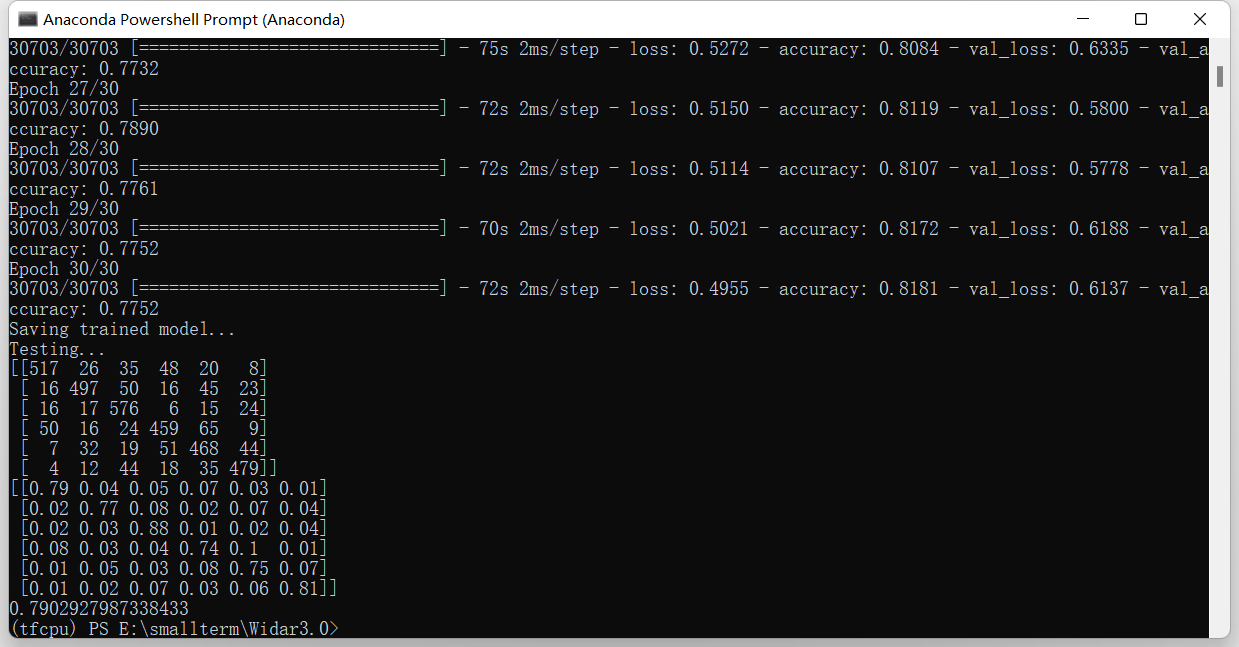
\includegraphics[width=16cm]{images/result.png}
                \captionsetup{font={small,bf,stretch=1.25}}
                \caption{训练结果}
                \label{fig1}
              \end{figure}
  上图展现了其中一次的深度学习输出结果,事实上tensorflow的random.set\_seed(1)的设置,导致该深度神经网络使用增益或权重的值每一次都会有所变化,因此每次训练结果的数值会有差别。在这一次的训练结果中,训练学习率达到了81.81\%,在随后的测试集中,给出了测试矩阵及测试结果,虽然测试准确率仅为79.03\%,较之前的学习准确率有所下降,但是在当时的研究现状上,跨域识别中准确率未曾有如此大的突破,可以证明BVP模块的思想是跨域识别中重要的贡献。 \par

\clearpage
\section{总结与心得}
\subsection{收获}
  在为期四周的小学期中,我阅读参考了一些关于无线感知和手势识别甚至人的其他点位识别的研究方式的文献,并与Widar3.0所论述的观点进行了简要的对比分析。并且在已有的环境基础之上,第一次亲自搭建了深度学习的环境,并且运用了功能强大的tensorflow keras框架,对深度学习的内容有了初步的认识。 \par
  在工具使用上,我学习了Emacs这一强大的专业编辑器,Emacs贯穿了小学期工作的始终,在使用体验上和上学期FreeBSD系统上的vim编辑器有类似的感受,两者都摆脱了对鼠标的依赖,虽然Emacs的快捷键组合复杂难记,但是在实际的使用过程中常用的一些操作渐渐了然于心。 \par
  Emacs不仅用于代码的编写和调整,还用于本报告的LaTeX编写,在这次小学期我第一次用LaTeX进行文档排版,LaTeX也是需要一定的代码数量,所以初次使用时会感到难以上手,在掌握了段落、编号、图片插入等基本操作后,文档的编写变得十分容易,并且可以直接编译成pdf文件,生成的文档整体简洁美观,我感受到了LaTeX排版文档的优势。
  \subsection{遇到的问题}
  小学期的一切领域和工具都是全新的,所以在完成工作中也是遇到了不少问题。 \par
  首先是环境安装的问题,Emacs本身是一个很好的编辑器,但是也需要一些插件的支持,所以配置文件的编写会遇到问题,Emacs启动时指定了配置文件的路线,所以配置文件的路径和命名是固定的。我多次创建了错误路径和错误命名的文件,导致即使Lisp代码安装的插件格式正确,在重启Emacs时也不会进行自动配置。在修改为正确的配置文件和匹配的镜像后,插件能够正确安装。 \par
  虽然查阅过资料得知keras、tensorflow、cuda、cudnn、python之间存在版本对应关系,但是组合的选取也比较困难,在开始的两周里尝试了若干种版本的组合,因为python的库函数和版本之间也有较强的依赖关系,经常遇到的情况是在花费大量时间安装了框架和依赖包后,发现使用的函数在现有的包中已不再适用,所以被迫重新选取所有包,不断地尝试、失败后才确定了一组合适的深度学习环境。 \par
  深度学习环境不兼容,Widar3.0所使用的训练环境和本机有所差距,所以要特别注重对硬件资源的把控。在运行程序时会跑满内存,导致很难进行其他的任何操作,然而即使这样,还是经常会出现内存、显存不足的情况,所以在每次运行程序时,需要手动设置虚拟内存的大小和分配方式。 \par
  还有Emacs和LaTeX工具的使用问题,相对于代码来说,工具的使用问题比较好处理,并且最后都能顺利解决。
  \subsection{对发展前景的展望}
  小学期中的跨域手势识别研究代表了2019年的成果,到如今已经过去了三年的时间,通过对该领域的洞察也发现有更多巧妙的手段能实现跨域的手势识别。随着无线感知技术的快速发展,越来越多的智能设备出现在市面上,手势识别这一人机交互方式被普遍认知是最简单、最轻松的。我们希望在不久的将来,手势识别能够像现在的人脸识别一样准确,并且相关的智能设备产品真正投入到每个百姓的家中使用。

 \clearpage
  \bibliography{ref}
\par
\par
\par
\par
\begin{center}
\textbf{Github项目地址} \\
\href{https://github.com/tian-apple/Smallterm}{https://github.com/tian-apple/Smallterm}

\end{center}

\end{document}